\begin{frame}{Lower bounds}


    $\varphi \only<4->{\alert{\xRightarrow[\hspace{1cm}]{} \text{dag-like communication}}}
    \only<2-4>{\xRightarrow[\hspace{1cm}]{} f_{\varphi}} \only<3-4>{\xRightarrow[\hspace{1cm}]{}
        \text{mon ckt. lower bounds}}
    \only<5->{\alert{\xRightarrow[\hspace{1cm}]{} \text{bottleneck counting}}}
    $


    \vspace{1cm}

    \pause
    $f_{\varphi}$ is hard for monotone circuits $\Rightarrow$ $\varphi$ is hard for CP
    \begin{itemize}
        \item{} [IPU 94, K96, P97] interpolation;
        \item{} [HP18, FPPR18] sertificate fo unsatisfiability.
    \end{itemize}

    \pause
    Monotone ckt. lower bounds
    \begin{itemize}
        \item{} [P97] approximation (clique);
        \item{} [HP18, FPPR18] Jukna's criteria.
    \end{itemize}

    \pause
    \pause
    \pause
    \vspace{1cm}
    \begin{theorem}
        For $c > 800$ whp any $\CP$-proof of random $c \log n$-CNF has size $2^{\Omega(n)}$.
    \end{theorem}
  
\end{frame}

\begin{frame}{Unsat clause search problem $\Search_{\varphi}$ (Lov{\'{a}}sz et al. 1994)}
    $\varphi(x, y)$ is an unsatisfiable CNF formula:
    \begin{itemize}
        \item Alice gets $a \in \{0, 1\}^n$;
        \item Bob gets $b \in \{0, 1\}^n$;
        \item goal: find a clause $C \in \varphi$, such that $C(a, b) = 0$.
    \end{itemize}

    \pause
    \vspace{1cm}

    \pause
    \begin{theorem}[Informal; Kraj{\'{\i}}{\v{c}}ek 98, Pudlak 99, S 17]
        There is a CP-proof of $\varphi$ of size $S$ $\Rightarrow$ dag-like protocol for
        $\Search_{\varphi}$ of size $S$.
    \end{theorem}
\end{frame}

\begin{frame}{Dag-like protocols}
    \vspace{-0.8cm}
    \begin{columns}[t]
        \begin{column}{0.58\textwidth}
            \begin{itemize}
                \item $H$ is a graph with out degree $2$, $\forall h \in H, ~ R_h \subseteq X \times Y$;
                \item $R_{\mathrm{root}} = X \times Y$;
                \item $a, b$ are children of $h$ $\Rightarrow$ $R_{h} \subseteq R_{a} \cup R_{b}$;
                \item $h$ is a leaf $\Rightarrow$ $h$ is marked by common solution for $R_h$.
            \end{itemize}
        \end{column}

		\begin{column}{0.38\textwidth}
            \begin{center}
                \tikzstyle{inner} = [thin, circle, minimum size = 0.3cm, draw, inner sep = 0.1pt, opacity = 1]

\tikzstyle{ed} = [thick, ->, draw, black, opacity = 1]

    
\begin{tikzpicture}[>=stealth']
    \node[inner] (a) at (0, 0) {};
    \node[inner] (b) at (-0.9, -0.7) {};
    \node[inner] (c) at (0.9, -0.7) {};
    \node[inner] (d) at (-1.5, -1.6) {\scriptsize $t_1$};
    \node[inner] (e) at (-0.3, -1.6) {};
    \node[inner] (f) at (1, -2) {};
    \node[inner] (g) at (-1.5, -3) {\scriptsize $t_2$};
    \node[inner] (h) at (-0.25, -3) {\scriptsize $t_3$};
    \node[inner] (g2) at (1.5, -3) {\scriptsize $t_3$};
    \node[inner] (h2) at (0.25, -3) {\scriptsize $t_2$};
    
    \path (a) edge[ed] (b);
    \path (a) edge[ed] (c);
    \path (b) edge[ed] (d);
    \path (b) edge[ed] (e);
    \path (c) edge[ed] (e);
    \path (c) edge[ed] (f);
    \path (e) edge[ed] (g);
    \path (e) edge[ed] (h);
    \path (f) edge[ed] (g2);
    \path (f) edge[ed] (h2);
\end{tikzpicture}

            \end{center}
		\end{column}
	\end{columns}

    \pause
    \begin{center}
        Rectangle (boolean) dag:
        
        \vspace{0.2cm}
        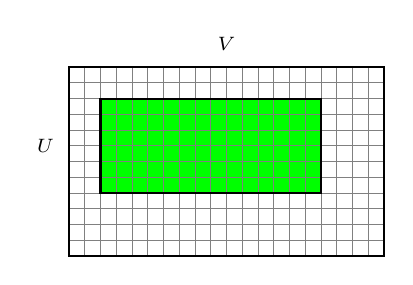
\begin{tikzpicture}
    \draw[fill = green] (0.4, -0.4) rectangle (3.2, -1.6);
    \draw[step = 0.2, gray, thin] (0, 0) grid (4, -2.4);
    \draw[black, thick] (0, 0) rectangle (4, -2.4);
    \draw[black, thick] (0.4, -0.4) rectangle (3.2, -1.6);
    \node at (-0.3, -1.) {\scriptsize $U$};
    \node at (2, 0.3) {\scriptsize $V$};
\end{tikzpicture}

    \end{center}

    We need \alert{triangles} instead of rectangles.

\end{frame}


\begin{frame}{Open Problems: Nisan--Wigderson Generators (naive encoding)}

    \begin{minipage}{0.48\linewidth}
        \centering
        \begin{tikzpicture}

    \pgfmathsetseed{1000007}
    \foreach \i in {0, 1, ..., 5}{
        \node[graph-vert] (b\i) at
            (1.5, 0.4 * \i + 0.4) {};
    }

    \foreach \i in {0, 1, ..., 7}{
        \node[graph-vert = {LEIorange!80!black}{0.15cm}] (a\i) at
            (0, 0.4 * \i) {};

        \draw[->] (a\i) -- ++(-0.3, 0);

        \foreach \j in {0, 1, 2}{
            \pgfmathsetmacro{\temp}{random(0, 5)}
            \draw (a\i) -- (b\temp);
        }
    }

    \node[below = 0.2cm] at (a0) {$m$};
    \node[below = 0.2cm] at (b0) {$n$};
\end{tikzpicture}
    \end{minipage}
    \putpos{-40}{50}{\includegraphics[scale = 0.1]{pics/utia-rest.png}}
    \begin{minipage}{0.48\linewidth}
        \begin{itemize}
            \item $\Delta$ is the left degree;
            \item $P(x_1, \dots, x_{\Delta})$ is a predicate.
        \end{itemize}
        
        \vspace{0.2cm}
        \pause
        \begin{itemize}
            \item Strategy do not work for balanced predicates;
            \item Upper bound if $P$ is $\Parity$;
            \item $\Ppoly$ vs $\NP$;
        \end{itemize}
    \end{minipage}
\end{frame}

\begin{frame}{Open problems}

    \begin{itemize}
        \item PRG. Other encodings.
        \item $\bigO{1}$-random CNF.
        \item ``Separation'' between CP and monotone circuits.
    \end{itemize}

    \vspace{1cm}
    \centering
    \includegraphics[scale = 0.1]{pics/utia-think.png}
\end{frame}